\section{Experiments}\label{sec:experiments}

We use two different convolutional architectures, each trained on the
ImageNet 2012 dataset \cite{imagenet}: PierreNet \cite{sermanet2013overfeat}, and MattNet \cite{zeiler2013visualizing}. 
We evaluate these networks on both CPU and GPU platforms. 

We now present results showing the performance of the approximations decribed in section \ref{sec:application} in terms of prediction accuracy, speedup gains and reduction in memory overhead. 

\vspace{-0.3cm}
\subsection{Speedup}
Table \ref{evaluation_time} shows the time breakdown of forward
propagation for each layer in MattNet. The majority of time is spent
in the first and second layer convolution operations, so restrict our
attention to these layers, although our approximations could easily
applied to convolutions in upper layers also.

We implemented several different approximation routines for the CPU
and as well as the GPU in an effort to achieve empirical
speedups. Both the baseline and approximation CPU code is implemented
in C++ using Eigen3 library \cite{eigenweb} compiled with Intel MKL.
We also use Intel's implementation of openmp, and multithreading. The
baseline gives comparable performance to highly optimized MATLAB
convolution routines and all of our CPU speedup results are computed
relative to this.  We used Alex Krizhevsky's CUDA convolution routines
\footnote{\url{https://code.google.com/p/cuda-convnet/}} as a baseline for GPU
comparisons. The approximation versions are written in CUDA. All GPU
code was run on a standard nVidia Titan card.

We have found that in practice it is often difficult to achieve
speedups close to the theoretical gains based on the number of
arithmetic operations.
Moreover, different computer architectures and convolutional network
architectures afford different optimization strategies making most
implementations highly specific.  However, regardless of
implementation details, all of the approximations we present reduce
both the number of operations and number of weights required to
compute the output by at least a factor of two.  While we present both
theoretical and empirical speedup results, the empirical aspects
serves largely as a proof of concept. Our aim is to illustrate that
the reduction in floating point operations and memory accesses that
are afforded by the approximations can in fact translate into speedups
in practice.  Our speedup results on both CPU and GPU are promising,
especially given that our baselines for comparison comprise of highly
optimized code. However, we believe that with extensive engineering
efforts, speedups can be much closer to theoretically optimal levels.

\begin{table}
\tiny
\parbox{.45\linewidth}{
\centering
\begin{tabular}{rrr}
\hline
Layer & Time per batch (sec) & Fraction \\
\hline
Conv1 & $2.8317 \pm 0.1030 $ & 21.97\% \\
MaxPool & $0.1059 \pm 0.0154$ & 0.82\% \\
LRNormal & $0.1918 \pm 0.0162$ & 1.49\% \\
Conv2 & $4.2626 \pm 0.0740 $ & 33.07\% \\
MaxPool & $0.0705  \pm 0.0029$ & 0.55\% \\
LRNormal & $0.0772\pm 0.0027$ & 0.60\% \\
Conv3 & $1.8689\pm 0.0577$ & 14.50\% \\
MaxPool & $0.0532\pm 0.0018 $ & 0.41\% \\
Conv4 & $1.5261\pm 0.0386$ & 11.84\% \\
Conv5 & $1.4222\pm 0.0416$& 11.03\% \\
MaxPool & $0.0102\pm 0.0006 $ & 0.08\% \\
FC & $0.3777\pm 0.0233$ & 2.93\% \\
FC & $0.0709  \pm 0.0038$ & 0.55\% \\
FC & $0.0168 \pm 0.0018$ & 0.13\% \\
Softmax & $0.0028 \pm 0.0015$ & 0.02\%\\
\hline 
Total & $12.8885$ & \\
\hline
\end{tabular}
}
\parbox{.45\linewidth}{
\centering
\begin{tabular}{rrr}
\hline
Layer & Time per batch (sec) & Fraction \\
\hline
Conv1 & $0.0604 \pm 0.0112$ & 5.14\% \\
MaxPool & $0.0072 \pm 0.0040$ & 0.61\% \\
LRNormal & $0.0041 \pm 0.0043$ &  0.35\% \\
Conv2 & $0.4663 \pm 0.0072$ & 39.68\% \\
MaxPool & $0.0032 \pm 0.0000$ &  0.27\% \\
LRNormal & $0.0015 \pm 0.0003$ & 0.13\% \\
Conv3 & $0.2219 \pm 0.0014$ & 18.88\% \\
MaxPool & $0.0016 \pm 0.0000$ & 0.14\% \\
Conv4 & $0.1991 \pm 0.0001$ & 16.94\% \\
Conv5 & $0.1958 \pm 0.0002$ &  16.66\% \\
MaxPool & $0.0005  \pm 0.0001$ & 0.04\% \\
FC & $0.0077 \pm 0.0013$ & 0.66\% \\
FC & $0.0017 \pm 0.0001$ & 0.14\% \\
FC & $0.0007 \pm 0.0002$  & 0.06\% \\
Softmax & $0.0038 \pm 0.0098$ & 0.32\%\\
\hline 
Total & 1.1752 & \\
\hline
\end{tabular}
}
\caption{Evaluation time in seconds per layer of MattNet on CPU (left)
  and GPU (right) with batch size of 128. Results are averaged over 8
  runs.} 
\label{evaluation_time}
\end{table}
\vspace{-0.8cm}

\subsubsection{First Layer}

The first convolutional layer in MattNet has 3 input channels, 96
output channels and 7x7 filters.  We approximated the weights in this
layer using the monochromatic approximation described in section
\ref{sec:application}. The monochromatic approximation works well if
the color components span a small number of one dimensional
subspaces. Figure \ref{fig:RGB_components} illustrates that by plotting the RGB components of the original filters and the filters after
projecting onto one dimensional subspaces. Figure \ref{fig:denoising} gives an alternate
presentation of this approximation, showing the original first layer
filters beside their monochromatic approximations.  Interestingly, we
notice that the approximated filters often appear to be cleaned up
versions of the original filters. This leads up to believe that the
approximation techniques presented ere might be viable strategies of
cleaning up or denoising weights after training, potentially to
improve generalization performance.

\begin{figure}[t]
\centering
\begin{minipage}{0.75\textwidth}
	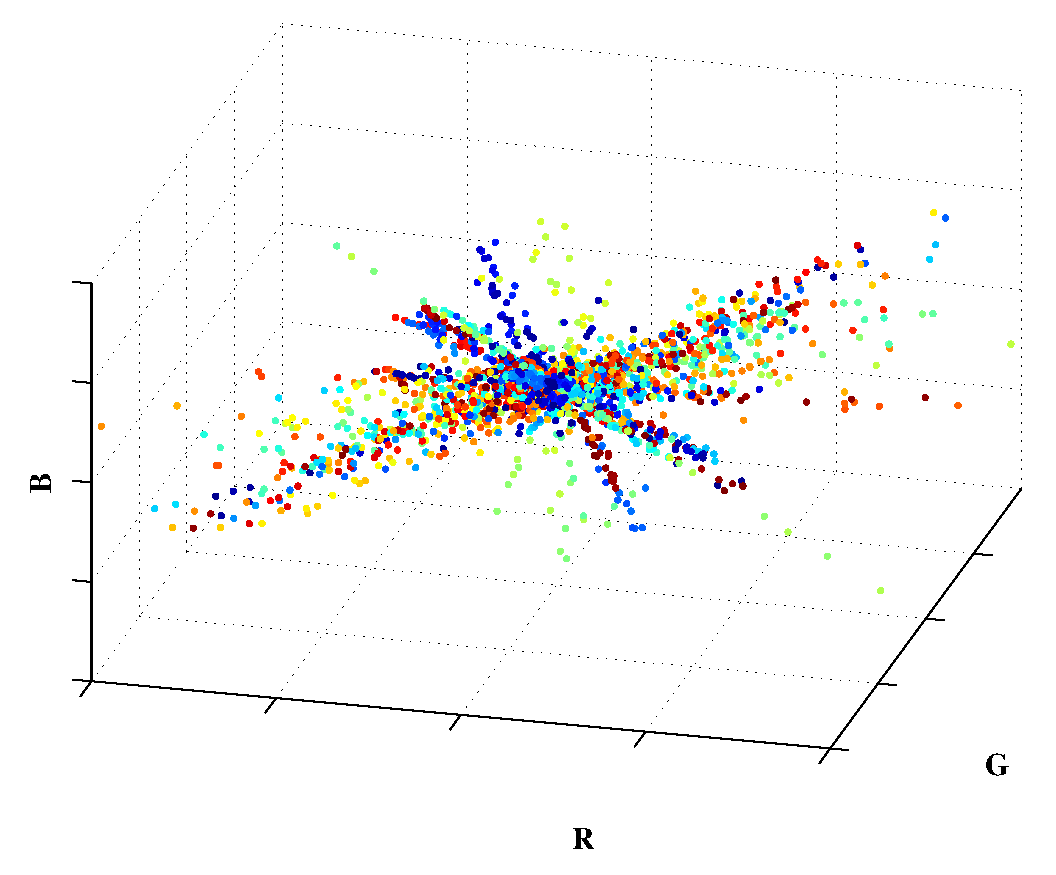
\includegraphics[width=0.5\linewidth]{img/RGB_components_matthew_3d.eps}
	\quad\quad
	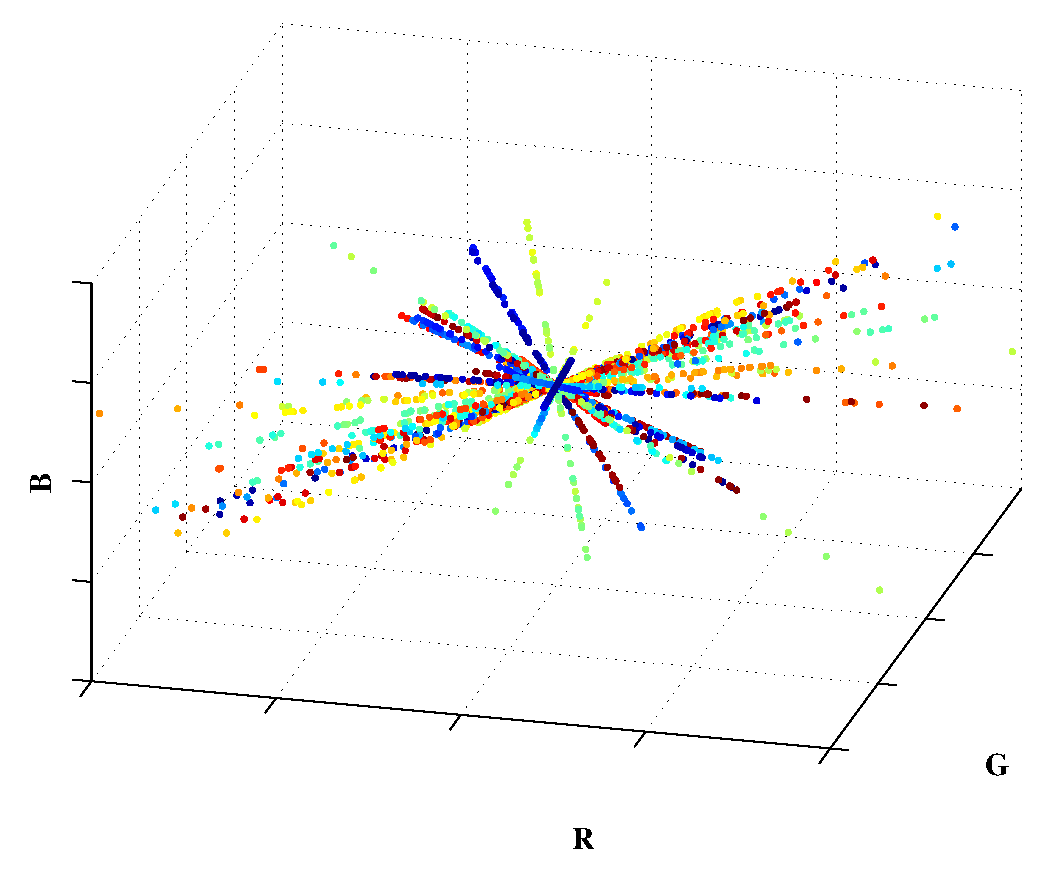
\includegraphics[width=0.5\linewidth]{img/monochromatic_RGB_components_matthew_3d.eps} 
\end{minipage}
\vspace{-3mm}
\label{fig:RGB_components}
\caption{Visualization of the 1st layer filters in MattNet. Each component of the 96 7x7 filters is plotted in RGB space. Points are colored based on the output filter they belong to. Hence, there are 96 colors and $7^2$ points of each color. ({\bf Left}) Shows the
  original filters and ({\bf Right}) shows the filters after the monochromatic approximation, where each filter has been projected down to a line in colorspace.}
\end{figure}



\begin{figure}[t]
\begin{center}
      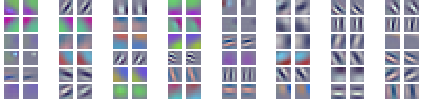
\includegraphics[width=0.9\linewidth]{img/denoising_combined.pdf}
\end{center}
\label{fig:denoising}
\vspace{-6mm}
\caption{Original and approximate versions (using 12 colors) of 1st later filters from MattNet.}
\end{figure}

We evaluated MattNet on 8K validation images from the ImageNet12 dataset using various monochromatic approximations for the first layer weights. The only parameter in the approximation is $C'$, the number of color channels used for the intermediate representation. As expected, the network performance begins to degrade as $C'$ decreases. Table \ref{table:mono_perf} shows how the classification performance degrades for increasing $C'$. 

\begin{table}[t]
\tiny
\centering
\begin{tabular}{ccc}
\hline
Number of colors \hspace{2mm} & Increase in test error & \hspace{2mm}Theoretical speedup\\
\hline
6 & 10.1929\% & 2.95$\times$ \\
8 & 4.0528\% & 2.94$\times$\\
12 & 2.1973\% & 2.91$\times$\\
16 & 1.1475\% & 2.88$\times$\\
24 & 1.7212\% & 2.82$\times$\\
48 & 0.5249\% & 2.66$\times$\\
96 & 0.5738\% & 2.39$\times$ \\
\hline 
\end{tabular}
\caption{Performance of MattNet when first layer weights are replaced with monochromatic approximation and the corresponding theoretical speedup. Classification error on 8K validation images tends to increase as the approximation becomes harsher (i.e. fewer colors are used). Theoretical speedups vary only slightly as the number of colors used increases since the color transformation contributes relatively little to the total number of operations.} 
\label{table:mono_perf}
\end{table}


Theoretically achievable speedups can measured in terms of the number of floating point operations required to compute the output of the convolution. 
For the monochromatic approximation this theoretical speedup with respect to MattNet is given in table \ref{table:mono_perf}. 
The majority of the operations result from the convolution part of the computation. In comparison, the number of operations required for the color transformation is negligible. Thus, the theoretically achievable speedup decreases only slightly as the number of color components used is increased. 

In practice, we found it difficult to optimize the monochromatic convolution routines as for large $C'$. Less work can be shared amongst output filters when $C'$ is large making it challenging to parallelize.
Figure \ref{fig:mono_speedups} shows the empirical speedups we acheived on CPU (left) and GPU (right) and the corresponding network performance for various numbers of colors used in the monochromatic approximation.   
Our CPU and GPU implementations achieve empirical speedups of $\sim1.8\times$ relative to the baseline with a drop in classification performance of less than 1.2\%. 

\begin{figure}[t]
\centering
\begin{minipage}{0.75\textwidth}
      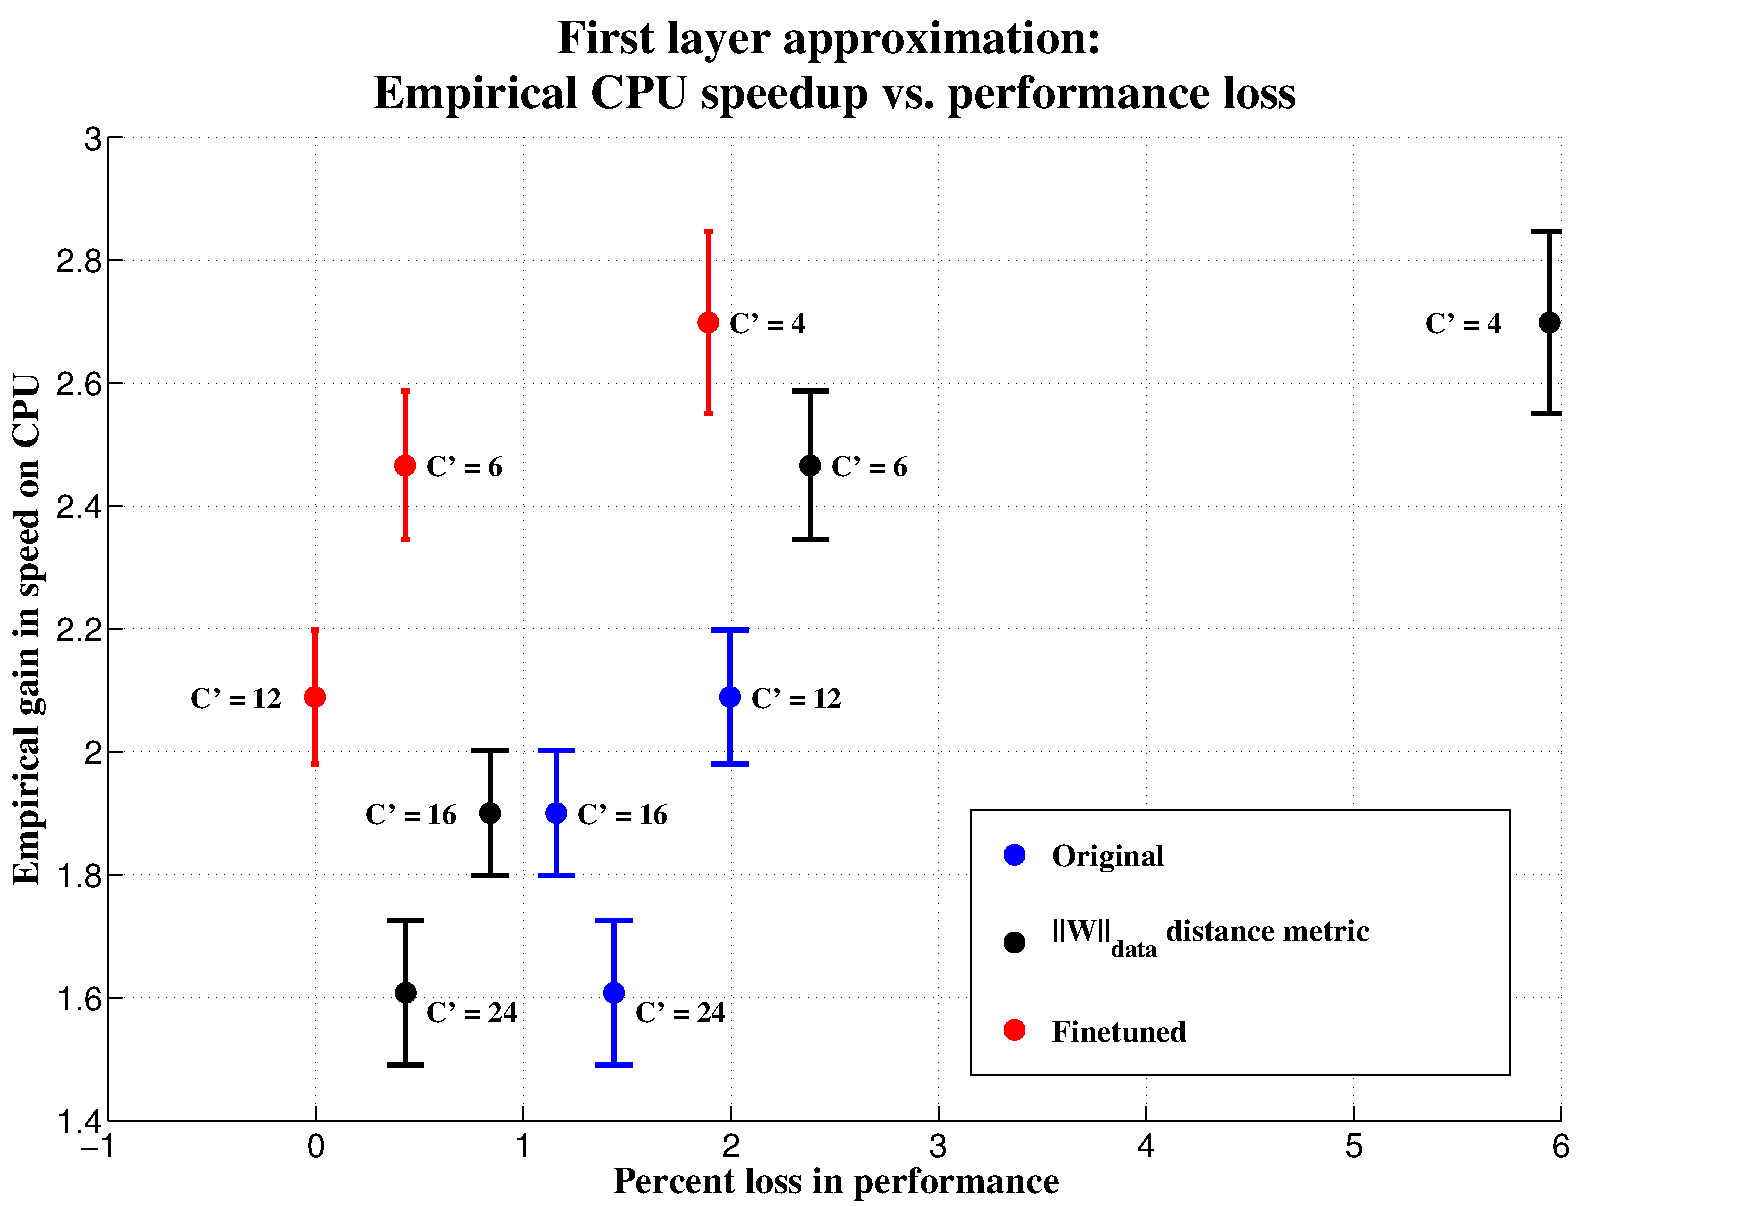
\includegraphics[width=0.5\linewidth]{img/layer1_CPUspeedup_vs_performance_loss_finetune_and_orig.pdf}
	\quad\quad
      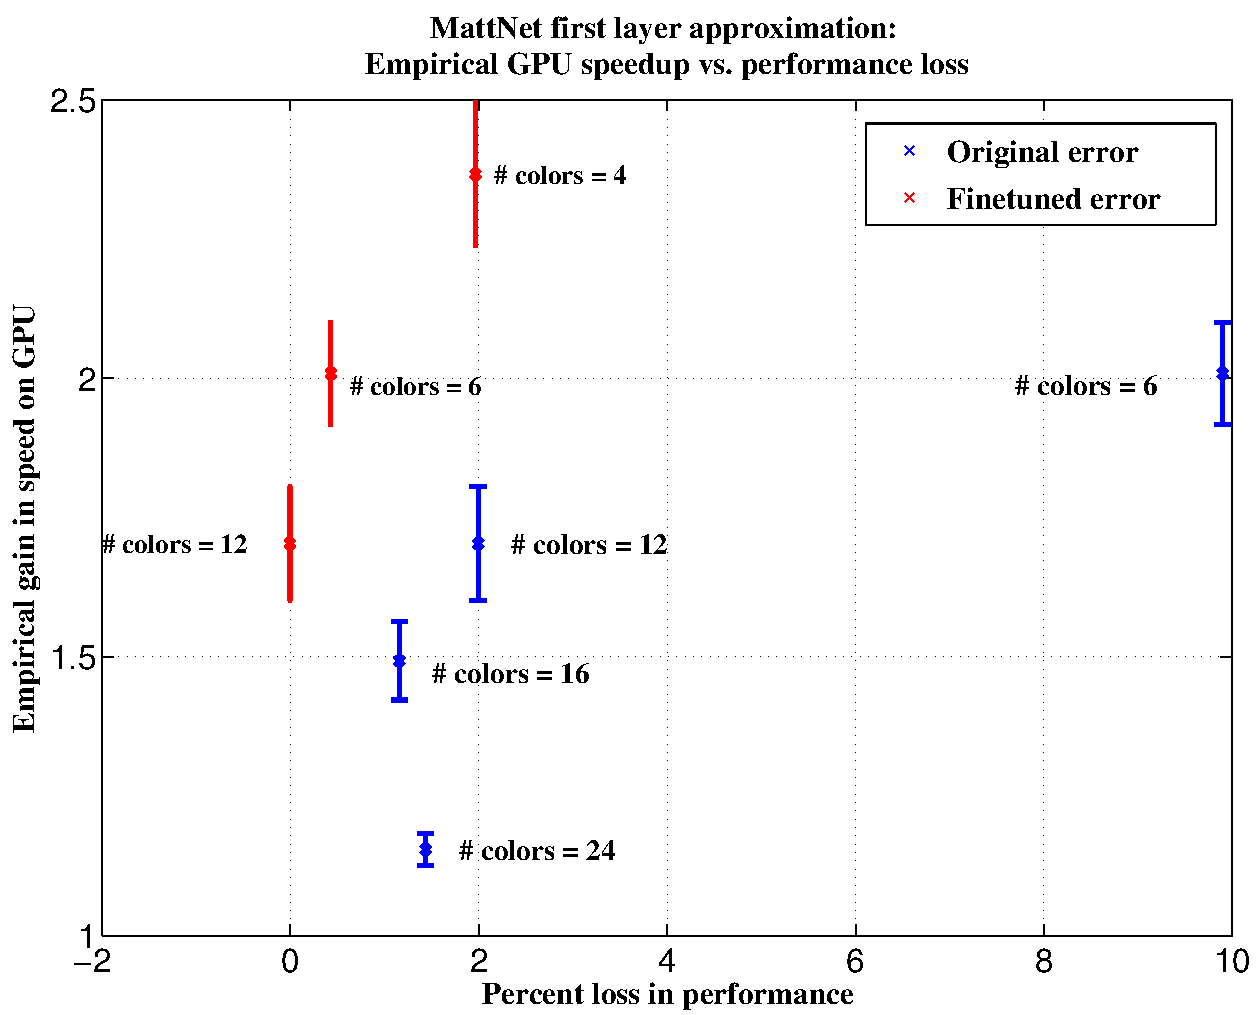
\includegraphics[width=0.5\linewidth]{img/layer1_GPUspeedup_vs_performance_loss_finetune_and_orig.pdf}
\end{minipage}
\caption{Empirical speedups on ({\bf Left}) CPU and ({\bf Right}) GPU for the first layer of MattNet.}
\label{fig:mono_speedups}
\end{figure}

\subsubsection{Second Layer}
The second convolutional layer in MattNet has 96 input channels, 256 output channels and 5x5 filters. 
We approximated the weights using the biclustering operation,
followed by the outer product decomposition approximation described in section \ref{sec:application}.
We evaluated the original and approximate convolution operation in
this layer using 8K validation images from the ImageNet12 dataset. 
We explored various configurations of the approximations by varying the number of input clusters $G$, the number of output clusters $H$ and the rank of the approximation. 

We can measure the theoretically achievable speedups for a particular approximation in terms of the number of floating point operations required to compute the output of the convolution. Figure \ref{fig:biclustering_theory} plots the theoretically achievable speedups against the drop in classification performance for various configurations.  
For a given setting of input and output clusters numbers, the performance tends to degrade as the rank is decreased. 

In practice we found it difficult to achieve speedups close to theoretically optimal levels. This is unsuprising given the amount of engineering effort that has gone into the baseline routines. However, we achieved promising results and present speedups of $\sim1.7\times$ relative to the baseline with less than a 1\% drop in performance.
Figure \ref{fig:biclust_speedups} shows our empirical speedups on CPU
(left) and GPU (right) and the corresponding network performance for
various approximation configurations. For the CPU implementation we used the biclustering with SVD decomposition approximation. For the GPU implementation we using the biclustering with outer product decomposition approximation.  
While we were unable to attain speedups on the order of those theoretically achievable, we are confident that further engineering efforts should decrease the margin.   

\begin{figure}[t]
\centering
\begin{minipage}{0.75\textwidth}
  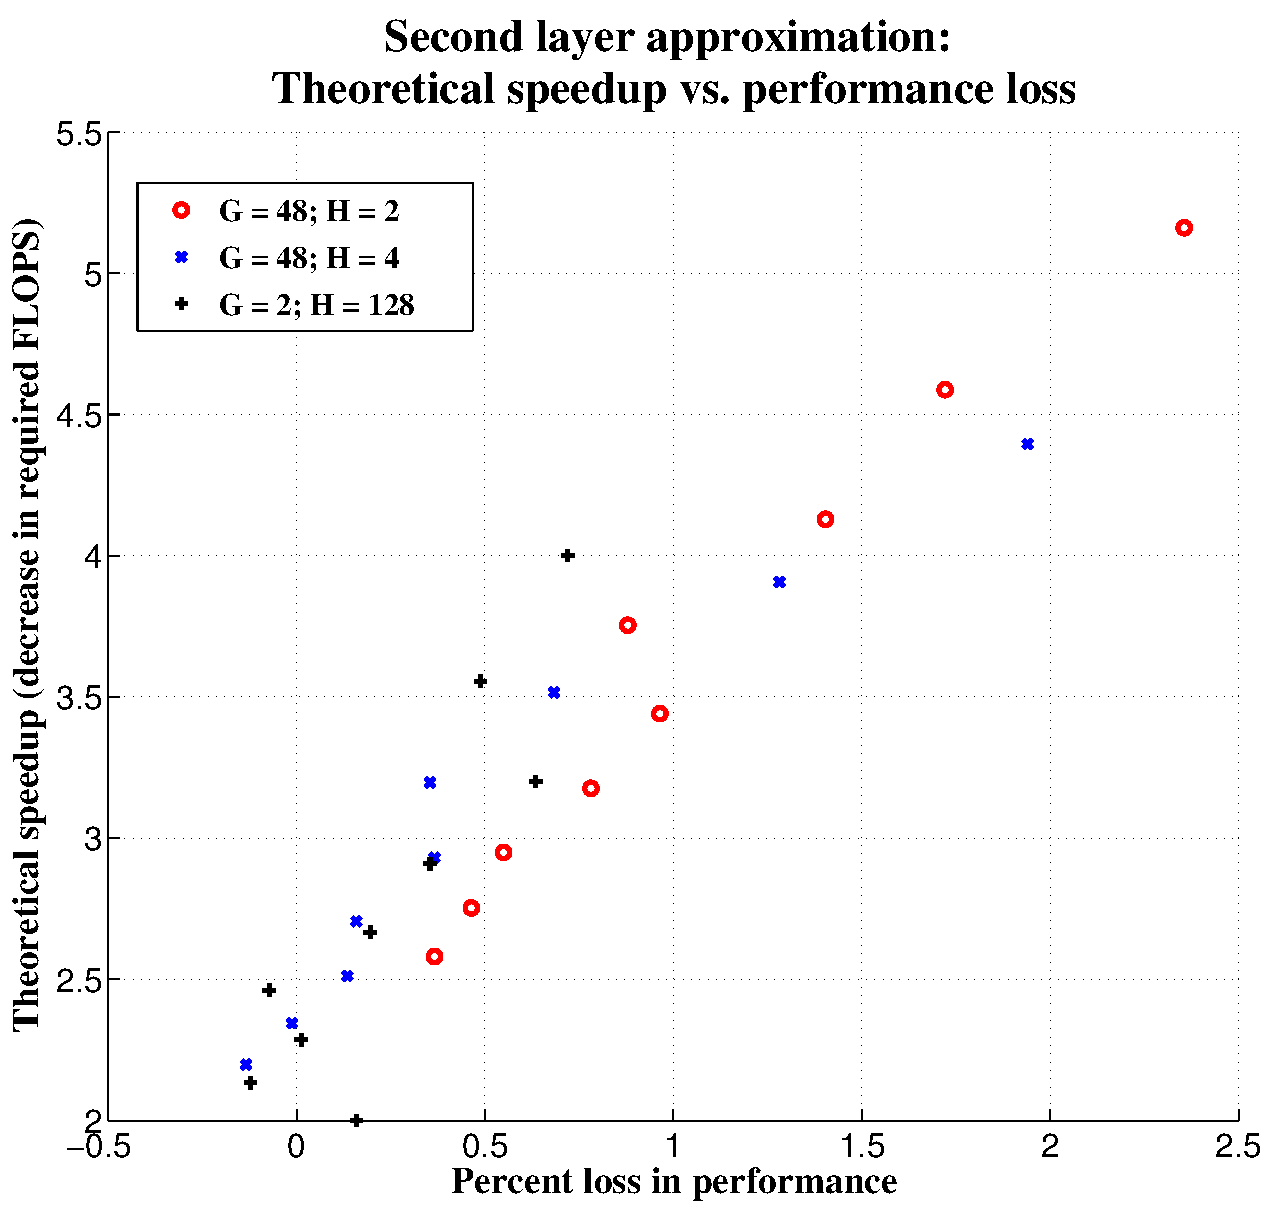
\includegraphics[width=0.5\linewidth]{img/layer2_theoreticalspeedup_vs_performance_loss.pdf} 
  \quad\quad
  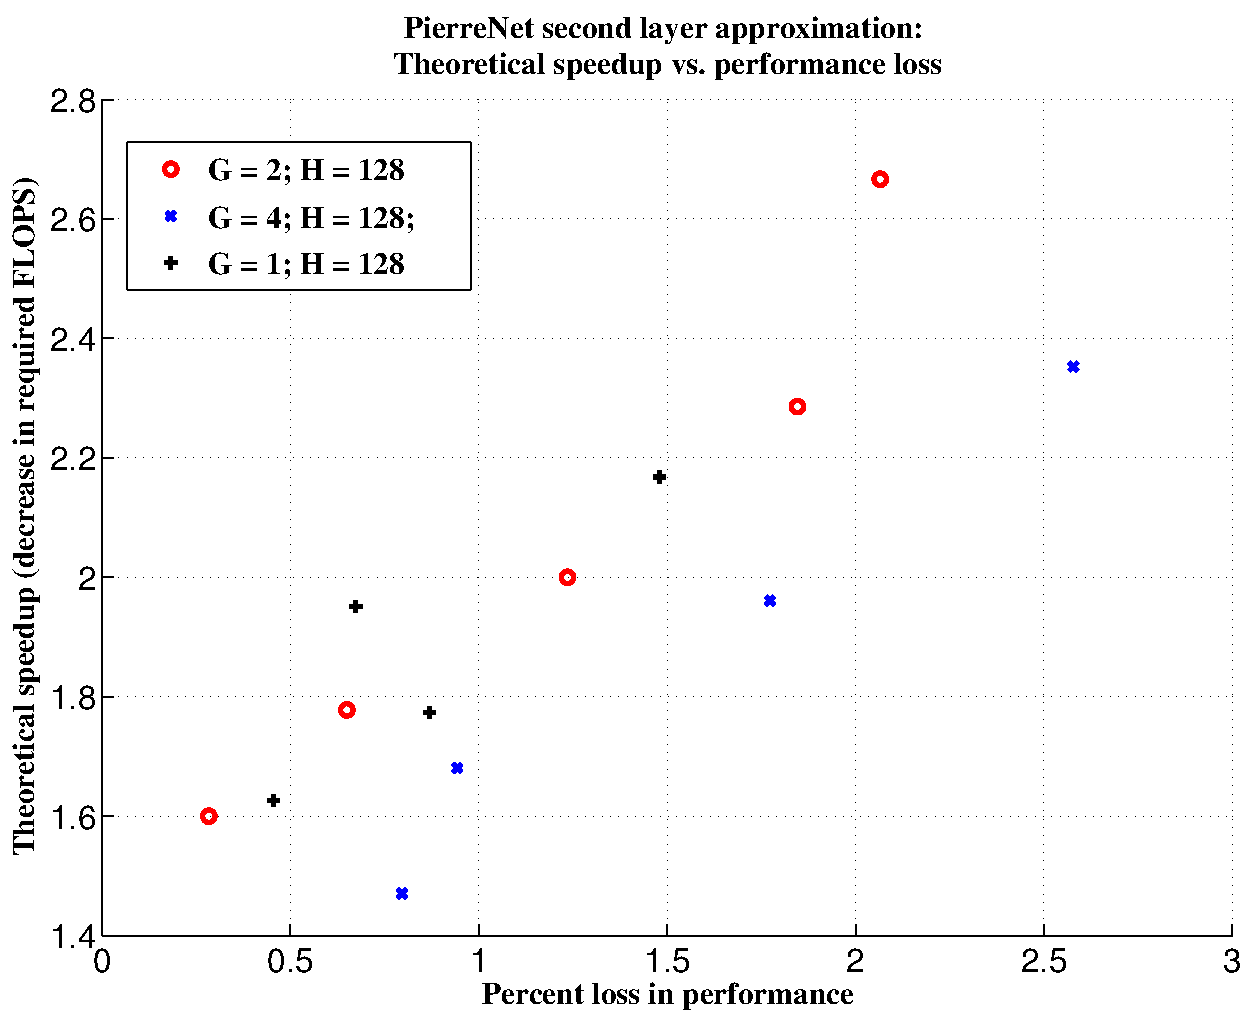
\includegraphics[width=0.5\linewidth]{img/layer2_theoreticalspeedup_vs_performance_loss_pierre.pdf} 
\end{minipage}
\caption{Theoretically achievable speedups with various biclustering approximations applied to ({\bf Left}) MattNet and ({\bf Right}) PierreNet.}
\label{fig:biclustering_theory}
\end{figure}

\begin{figure}[t]
\centering
\begin{minipage}{0.75\textwidth}
      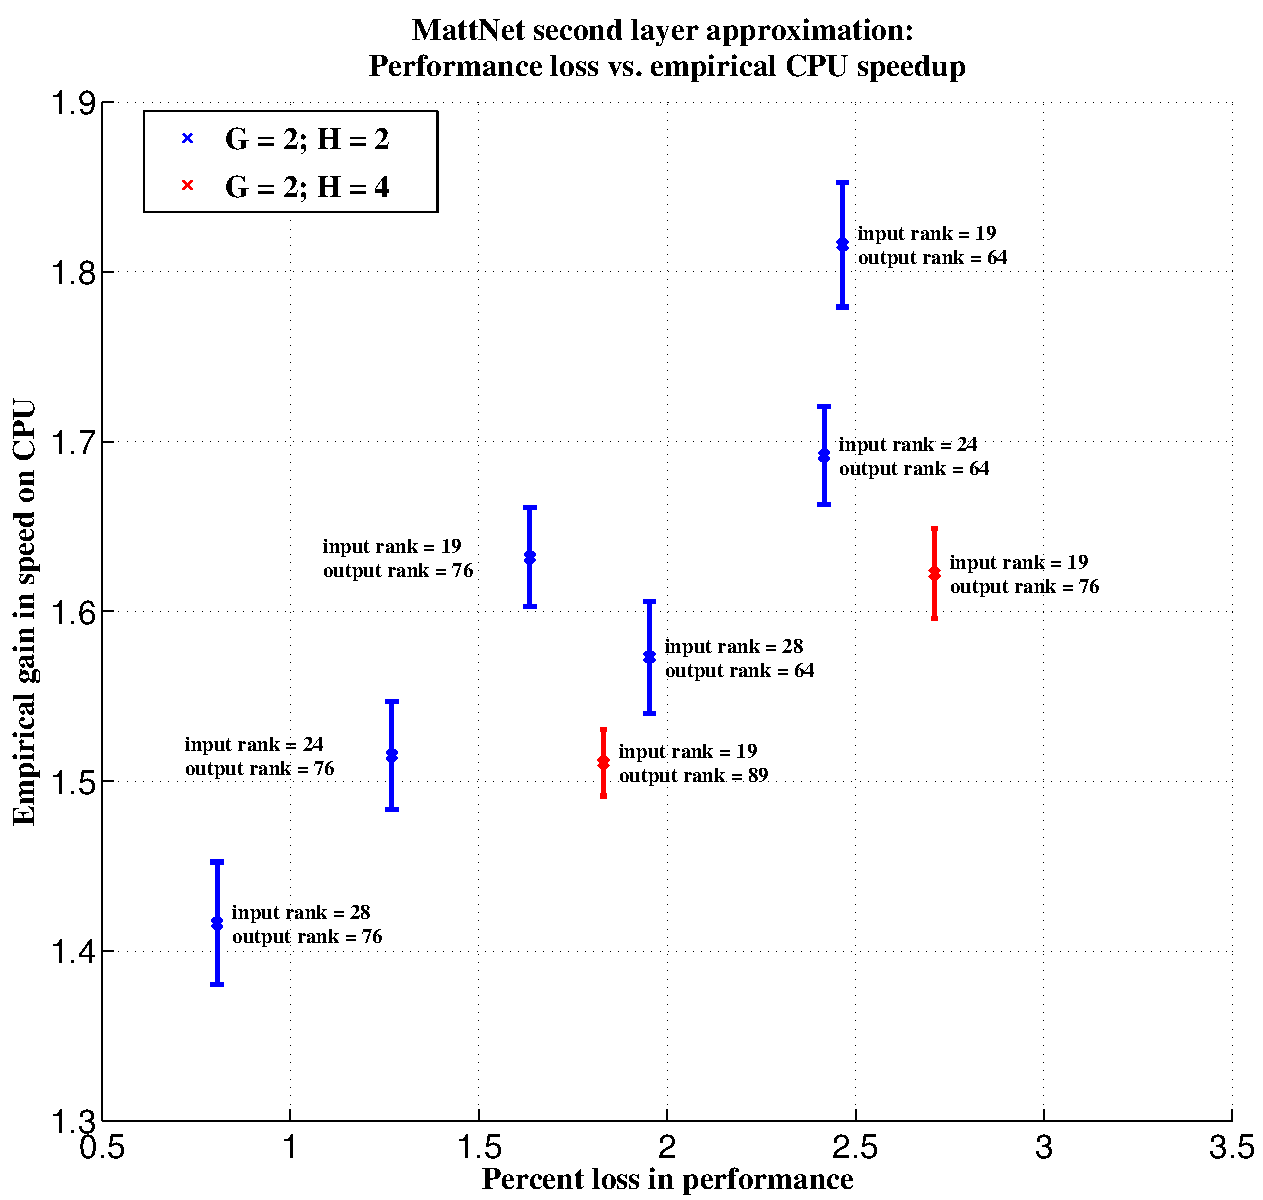
\includegraphics[width=0.5\linewidth]{img/layer2_CPUspeedup_vs_performance_loss.pdf}
      \quad\quad
      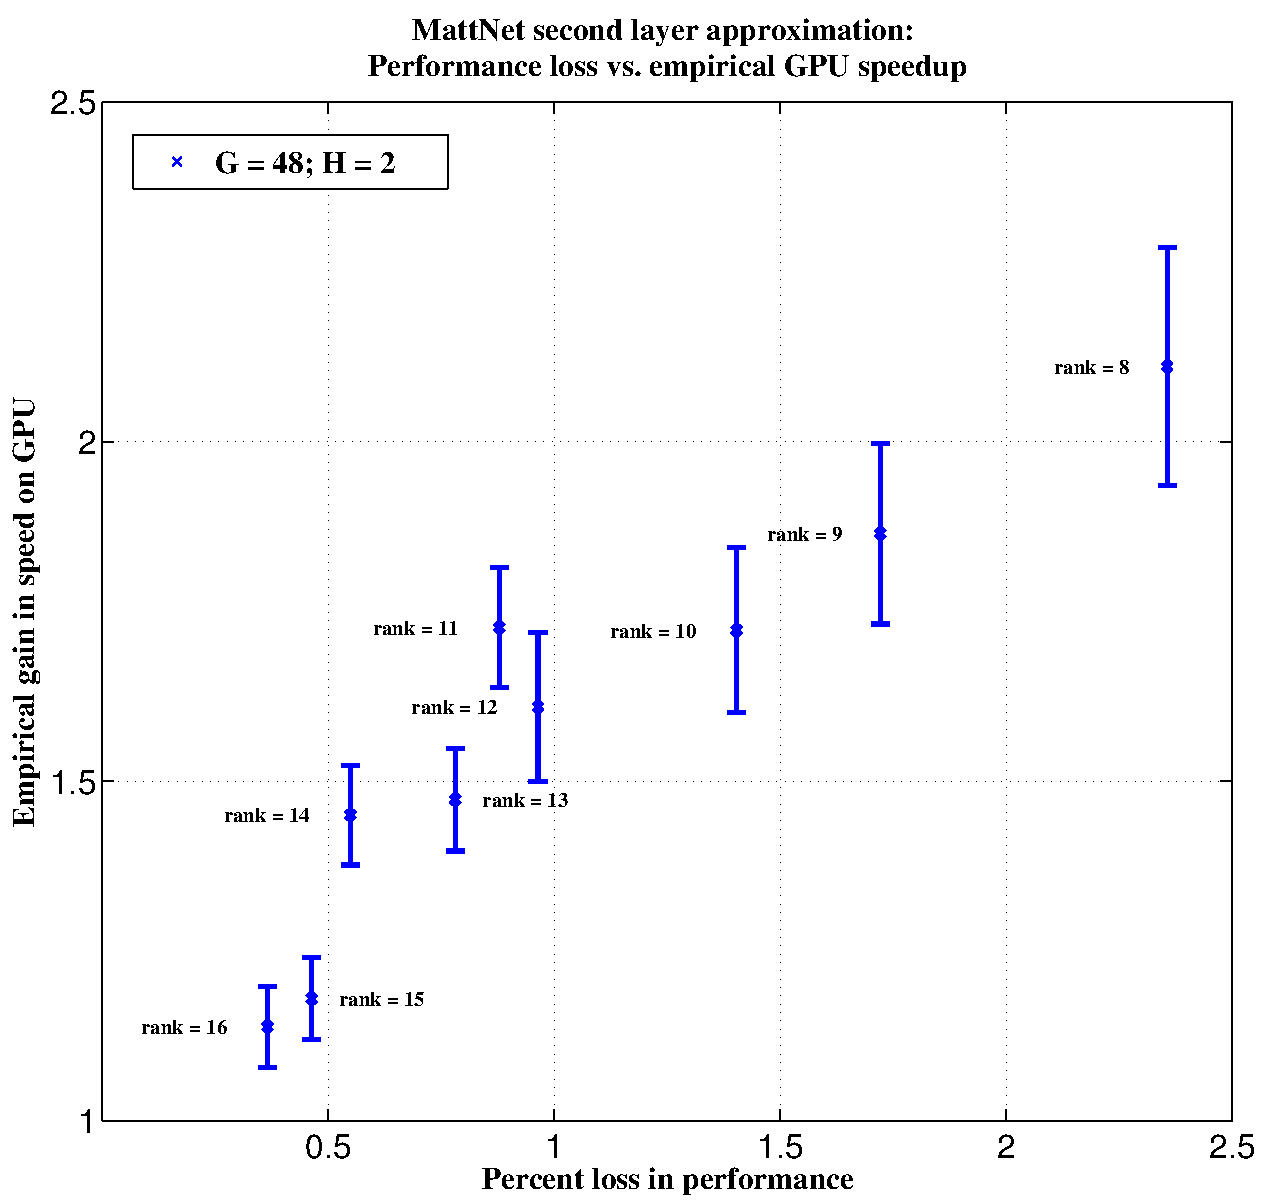
\includegraphics[width=0.5\linewidth]{img/layer2_GPUspeedup_vs_performance_loss.pdf}
\end{minipage}
\caption{Empirical speedups on ({\bf Left}) CPU and ({\bf Right}) GPU for the second layer of MattNet.}
\label{fig:biclust_speedups}
\end{figure}


\subsection{Reduction in memory overhead}
In many commercial applications memory conservation and storage are a
central concern. This mainly applies to embedded systems
(e.g. smartphones), where available memory is limited, and users are
reluctant to download large files. In these cases, being able to
compress the neural network is crucial for the viability of the
product. 

In addition to requiring fewer operations, our approximations
require significantly fewer parameters when compared to the original
model. Table \ref{table:memory_theory} shows the number of parameters for
various approximation methods as a function of hyperparameters for the approximation techniques. Table \ref{table:memory_empirical} shows the empirical reduction of parameters for MattNet and the corresponding network performance.

\begin{table}[t]
\tiny
\centering
\begin{tabular}{cc}
\hline
Approximation method & Number of parameters \\
\hline
No approximation & $C \cdot X \cdot Y \cdot F$\\
Monochromatic & $C \cdot C' + X \cdot Y \cdot F$\\
Biclustering + outer product decomposition & $G \cdot H \cdot K (\frac{C}{G} + X \cdot Y + \frac{F}{H})$ \\
Biclustering + singular value decomposition & $G \cdot H \cdot (\frac{C}{G} \cdot K_1 + K_1 \cdot X \cdot Y \cdot K_2 + K_2 \cdot \frac{F}{H})$ \\
\hline 
\end{tabular}
\caption{Number of parameters expressed as a function of hyperparameters for various approximation methods.} 
\label{table:memory_theory}
\end{table}

\begin{table}[t]
\tiny
\centering
\begin{tabular}{lccc}
\hline
Approximation method &Approximation hyperparameters &  Reduction in weights & Increase in test error\\
\hline
\hline
Layer 1: Monochromatic & $C' = 48$ & 2.9109$\times$ & 0.5249\%\\
\hline
Layer 2: Biclustering & $G = 48$ & 3.7537$\times$ & 0.8789\%\\
	    +outer product decomposition & $H = 2$ & & \\
								     & $K = 11$ & & \\
\hline
Layer 2: Biclustering & $G = 2$ & 2.0386$\times$ & 0.8057\% \\
	  + singular value decomposition	& $H = 2$ & &\\
										& $K_1 = 28$ & &\\
										& $K_2 = 76$ & &\\
\hline 
\end{tabular}
\caption{Empirical reduction in parameters for first two layers of MattNet with corresponding network performance.} 
\label{table:memory_empirical}
\end{table}

